\chapter{Исследовательская часть}

\section{Технические характеристики}

Технические характеристики устройства, на котором выполнялось тестирование:
\begin{itemize}
	\item операционная система: Ubuntu 22.04.1 LTS Linux x86\_64 \cite{ubuntu};
	\item память: 8 ГБ;
	\item процессор: Intel® Core™ i3-7130U.
\end{itemize}

Тестирование проводилось на ноутбуке, включенном в сеть электропитания. Во время тестирования ноутбук был нагружен только встроенными приложениями окружения, окружением, а также непосредственно системой тестирования.

\section{Пример работы программы}

На рисунке \ref{img:example} представлен пример работы программы. Вводится размерность массива и элементы массива. Далее выводится отсортированный массив и время выполнения каждой сортировки в микросекундах. Все сортировки верно отсортировали исходный массив.  
В данном примере:
\begin{itemize}
	\item присутствовали отрицательные элементы (дополнительный массив в сортировке подсчетом был размерности 16, что больше размера самого массива);
	\item размер массива не равен степени числа два (для битонной сортировки массив дополнялся фиктивными элементами);
	\item максимальный и минимальный элементы находились в конце (худший случай поиска минимального и максимального элементов в сортировке подсчетом).
\end{itemize} 

\begin{figure}[h]
	\centering
	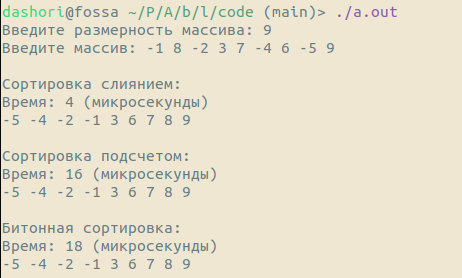
\includegraphics[width=130mm]{images/example}
	\caption{Пример работы программы}
	\label{img:example}
\end{figure}

\section{Время выполнения реализованных алгоритмов}

Замеры времени работы реализованных алгоритмов для массива каждой размерности проводились 2000 раз. Все три алгоритма сортировки имеют одинаковую трудоемкость в лучшем, худшем и среднем случаях, поэтому каждый раз элементы массива генерировались случайно -- числа из диапазона (-INT\_MAX, INT\_MAX) \cite{si}. Данный диапазон исключает превосходство сортировки подсчетом из-за входных данных, так как дополнительный массив явно содержал больше элементов, чем исходный. В качестве результата, представленного в таблице \ref{tab:time}, взято среднее время на каждой длине массива.
\clearpage
\begin{table}
	\begin{center}
		\caption{\label{tab:time}Результаты замеров времени реализованных сортировок в микросекундах}
	\begin{tabular}{|l|l|l|l|l|}
		\hline \specialcell{Длина массива} & \specialcell{Слиянием\\} &
		 \specialcell{Подсчетом} & \specialcell{Битонная} \\\hline
		10 & 1 & 1 & 2 \\ \hline
		30 & 2 & 1 & 8 \\ \hline
		64 & 2 & 1 & 8 \\ \hline
		128 & 6  & 1  & 23 \\ \hline
		200 & 10 &  2 &  56 \\ \hline
		254 & 12 & 3 & 57 \\ \hline
		255 & 12 &  3 &  57 \\ \hline
		256 & 12 &  3 &  55 \\ \hline
		257 & 13 &  3 &  131   \\ \hline
		258 & 13 & 3 & 131 \\ \hline
		300 & 16 &  3 &  136 \\ \hline
		400 & 22 &  4 &  134 \\ \hline
		500 & 27 &  5 &  136 \\ \hline
		512 & 27 &  5 &  133 \\ \hline
		1024 & 59  & 11  & 316 \\ \hline
		2048 & 128 &  22 &  736 \\ \hline
		4096 & 272 &  45 &  1696 \\ \hline
		8192 & 573 &  90 &  3856  \\ \hline
		16384 & 1197 & 181 & 8720 \\ \hline
		32768 & 2502 & 363 & 19570 \\ \hline
		65536 & 5229 & 726 & 43674 \\ \hline
	\end{tabular}
	\end{center}
\end{table}
На рисунке \ref{img:result} представлена зависимость времени работы реализованных алгоритмов сортировки от длины массива. На рисунке \ref{img:resultDegree} представлена зависимость времени работы реализованных алгоритмов сортировки от длины массива, где длина массива -- степень числа два.

\begin{figure}[h]
	\centering
	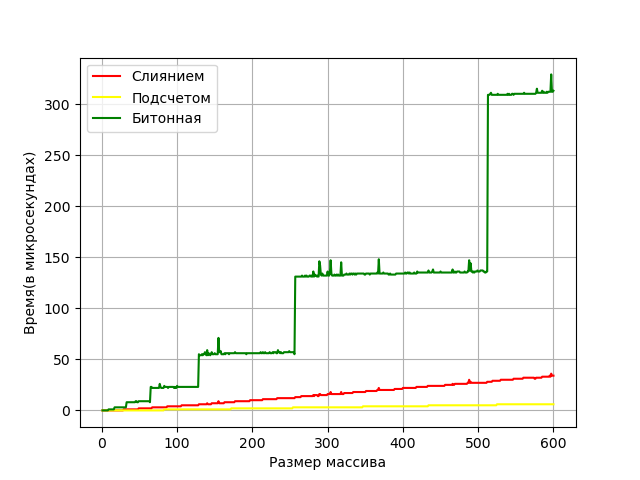
\includegraphics[width=140mm]{images/result}
	\caption{Зависимость времени работы реализованных алгоритмов сортировки от длины массива.}
	\label{img:result}
\end{figure}
\begin{figure}[h]
	\centering
	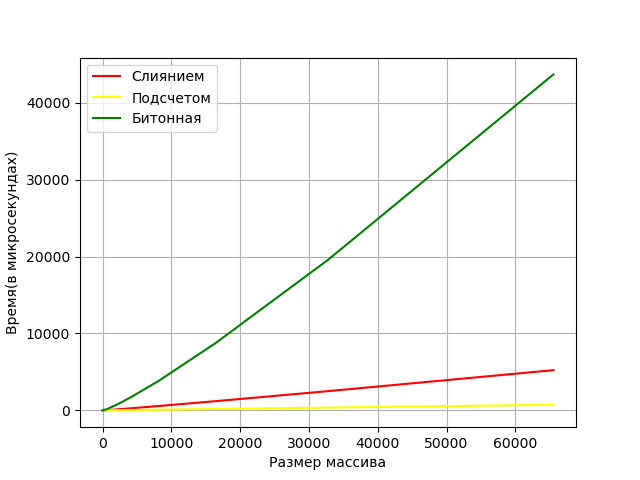
\includegraphics[width=140mm]{images/resultDegree}
	\caption{Зависимость времени работы реализованных алгоритмов сортировки от длины массива, где длина -- степень числа два.}
	\label{img:resultDegree}
\end{figure}

\clearpage
Из рисунка \ref{img:result} видно особенность битонной сортировки, которая сортирует только массивы, длина которых является степенью числа два. Все массивы, имеющую иную длину, дополняются фиктивными элементами до ближайшей степени числа два, что видно на рисунке \ref{img:result}. 

Самая быстрая сортировка из исследуемых -- сортировка подсчетом. На размерах массива до 64 она превосходит в 8 раз битонная сортировка и в 3 раза сортировка слиянием. На размерах от 100 до 600 она работает быстрее в 30-50 чем битонная и в 6 раз быстрее чем сортировка слиянием.
На самом максимальном тестируемом размере -- 65536 сортировка подсчетом быстрее битонной сортировки в 60 раз, а сортировки слиянием в 7 раз.  

Быстрая скорость сортировки подсчетом объясняется тем фактом, что она проигрывает по памяти двум другим алгоритмам сортировки, так как хранит дополнительный массив длина которого -- диапазон значений. Так как значения элементов массива генерировались произвольно в диапазоне (-INT\_MAX, INT\_MAX) \cite{si}, исключается вариант, что сортировка подсчетом работает быстрее из-за тестовых данных. Также алгоритм битонной сортировки был реализован не параллельно, что ухудшает его трудоемкость.

